To predict punctuations in unformatted text, we use two different models: a lexical model, which is based on lexical features, and an acoustic model, which is based on prosodic features.
For our approach we used a deep learning approach using the deep learning framework \emph{Caffe}\footnote{http://caffe.berkeleyvision.org/}.
In this chapter we describe how we predict the position of periods and commas in unpunctuated text using lexical features.

\subsection{Training Instance Generation}
For training our lexical model we took the \texttt{.xml} files of the TED talks and the Wikipedia files.
Before we can train the neural network with \emph{Caffe}, we have to preprocess the data to generate the training instances.
An overview of the individual steps for creating the training instances from the input files is shown in Figure~\ref{fig:overview_lexical}.

\begin{figure}[ht]
    \centering
    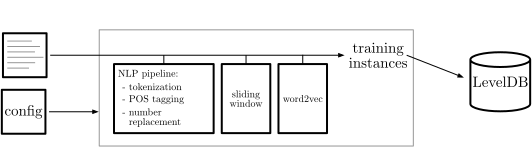
\includegraphics[width=0.7\textwidth]{img/overview_lexical.pdf}
    \caption{Creation of the training instances for the lexical model: The input text is tokenized, the POS tags are determined, and numbers are replaced. Then, a sliding window is used to create the training instance. Each word is thereby replaced with a distributed word representation.}
    \label{fig:overview_lexical}
\end{figure}

In a first step the plain text from the input files is extracted.
The input text is formatted, i.e., it contains all kinds of punctuation marks.
We can use this information as our gold standard.
We use the following two classes: \textsc{Period} and \textsc{Comma}.
The class \textsc{Period} is mapped to the following characters: ``;'', ``.'', ``!'' and ``?''.
The characters ``,'', ``:'' and ``-'' are mapped to the class \textsc{Comma}.
If there is no punctuation, we use the class \textsc{None}.

Once we have the input text, the next step is the tokenization.
Afterwards, we run a sliding window over the input text to create the training instances.
The sliding window procedure is illustrated in Figure~\ref{fig:sliding_window}.
\begin{figure}[ht]
    \centering
    
\includegraphics[width=0.8\textwidth]{img/sliding_window.pdf}
    \caption{Training instances from sliding window: Each window constitutes one training instances. The length of the window and the position, which determines the label, is a parameter. In the example we use a window size of five and the punctuation position three.}
    \label{fig:sliding_window}
\end{figure}
The size of the window is determined by a \texttt{config} file.
The \texttt{config} file stores different parameters, which are used during the process of generating the training instances.
Having those \texttt{config} files makes it easy to generate different kind of training instances and therefore to evaluate different configurations.
The window size directly defines the size of the training instance.
The label of a training instance is determined by whether there is a punctuation at a certain position or not.
This position is also defined in the \texttt{config} file and is called punctuation position.
If there is no punctuation at this position, the label of the training instance would be 0 (stands for class \textsc{None}), if there is one character of the class \textsc{Comma}, it would be 1, and if it is a character of the class \texttt{Period}, the label would be 2.

After we divide the sentences into training instances, we convert each word into a distributed word representation.
This step is necessary to obtain a representation of the words, which the neural network can learn from.
The implementation of the distributed representation we use is \emph{word2vec}~\cite{Mikolov1, Mikolov2, Mikolov3}.
More precisely, we use a pretrained vector file\footnote{\url{https://code.google.com/archive/p/word2vec/}}, which was trained on a Google News data set.
The model contains 300-dimensional word vectors for three million different words and phrases.

Since not every word exists in the trained model, we use the word vector representing \texttt{this} for unknown words.
We think that most of the unknown words are proper names, which can be replaced with \texttt{this} without changing the meaning and structure of the entire sentence.
Besides, the trained model contains only a few numbers.
As the concrete number occurring in a text is not relevant for the sentence boundary detection, we replace all numbers in the text, including floating-point numbers, with the number 1.
The representation for each word in a training instance is inserted into one row of the feature matrix, e.g., for a sliding window size of five a matrix of size 5x300 for each training instance is generated.

In addition to the distributed word representation, we also examined Part of Speech (POS) tags as features.
Therefore, we used the \emph{nltk}\footnote{\url{http://www.nltk.org/}} POS tagger.
The tagger distinguishes between 35 different POS tags.
These are too specific for our purpose, so we grouped them into 14 different categories.
For example, there exist four different tags, which identify a noun.
The \emph{nltk} tagger predicts more than one tag per word, so one word can have multiple tags (even after reducing the tag categories).
To allow the existence of multiple tags in our feature matrix, we used the following representation:
We create one flag per POS category, which has the value 1 if the word belongs to this category and 0 otherwise.

One can think of several strategies to include the POS features in the training instances.
We decided for the most straightforward: appending the features after the word vector representation, thus resulting in a feature matrix of 5x314 for a sliding window size of five with POS tags.

The created training instances are written to a LevelDB in a last step.
Using the LevelDB, we can now train our neural network.

\subsection{Neural Network Layout}

The layout of our neural network is shown in Figure~\ref{fig:net_lexical}.
\begin{figure}[ht]
    \centering
    
\includegraphics[width=0.6\textwidth]{img/net_lexical.pdf}
    \caption{Network architecture consisting of four \texttt{inner product} layers.}
    \label{fig:net_lexical}
\end{figure}
We use a neural network layout with three main \texttt{inner product} layers with sizes 2048, 4096, and 2048.
After each of these layers we added a \texttt{ReLU} and a \texttt{dropout} layer on top of each \texttt{inner product} layer.
The ratio for all \texttt{dropout} layers is 0.5.
Accuracy and loss of the network are computed after the final predictions of our fourth \texttt{inner product} layer with size 3.

\subsection{Results and Evaluation}

As one evaluation metric we use F-measure, which is based on precision \emph{P} and recall \emph{R} as seen in Equation~\ref{equ:f1n}.
The F-measure can be calculated for each class (\textsc{None}, \textsc{Period}, \textsc{Comma}).
To obtain a single metric for the performance in all three classes, we use the generalized form of the F-measure, the harmonic mean (see Equation~\ref{equ:f1}).
The higher the value, the better.
The F-score is used as evaluation metric for all our experiments.
\begin{equation}
\label{equ:f1n}
F1_{None} = 2 * \frac{P_{None}* R_{None}}{P_{None}+R_{None}}
\end{equation}
\begin{equation}
\label{equ:f1}
F-score = \frac{3}{\frac{1}{F1_{None}} + \frac{1}{F1_{Comma}} + \frac{1}{F1_{Period}}}
\end{equation}

All experiments are executed with the previously described data preprocessing and network layout.
As test data we used TED talks from 2011, which we did not include in the training set.

In a first experiment, we examined if training on TED talk data together with the Wikipedia data improves the performance. 
In Figure~\ref{fig:window_wiki_eval} we show a comparison between using only TED talks and using additional Wikipedia data as training data.
\begin{figure}[ht]
    \centering
    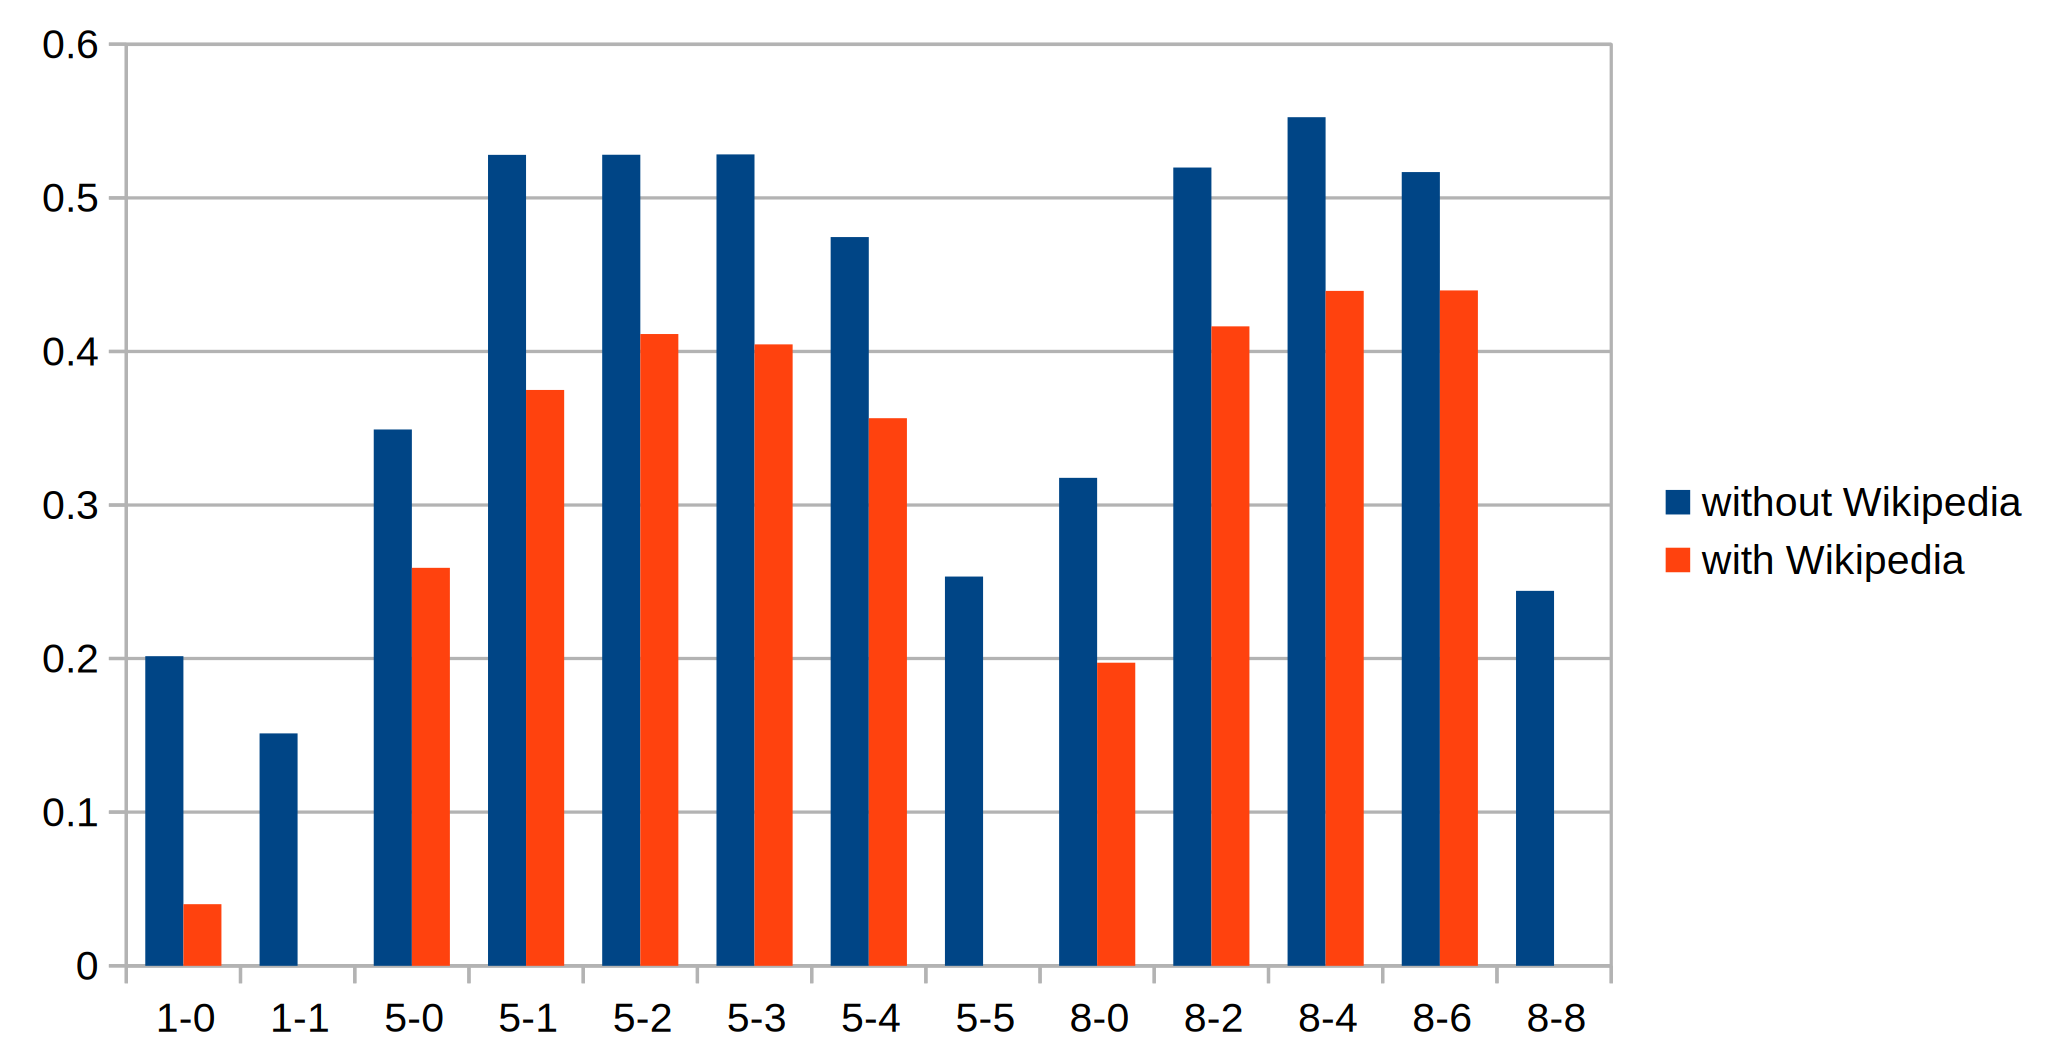
\includegraphics[width=0.7\textwidth]{img/window_wiki_eval.png}
    \caption{Results for different training data: The blue bars stands for a training set consisting only of TED talks, the red bars represents a training set based on TED talks and Wikipedia articles. The F-score is plotted against different window sizes and punctuation positions. The results show, that using Wikipedia as training data decreases the performance.}
    \label{fig:window_wiki_eval}
\end{figure}
The F-score on the y-axis is plotted against different window sizes and punctuation positions on the x-axis.
\texttt{5-3} on the x-axis means, that we have a window size of five and a punctuation position of three.
The blue bars display the result for training without Wikipedia, the red bars are the results, where Wikipedia was included in the training data set.
The results show, that using Wikipedia data as additional training data always performs worse.

It seems that adding more training data in form of Wikipedia articles does not help to increase the performance when evaluating on TED talks.
Our hypothesis is, that the speech from TED talks is fundamentally different from the formal, written Wikipedia articles.
We can confirm this hypothesis by not evaluating on TED talks, but rather on different Wikipedia articles.
In that case, adding Wikipedia articles to the training data set increased the F-score by 6\%, overall yielding an F-score of 60\%.
For segmenting ASR output, we therefore do not use additional Wikipedia data for prediction.

We also evaluated whether POS tags improve the results.
Figure~\ref{fig:window_pos_eval} shows the F-score depending on the different window sizes and punctuation positions.
\begin{figure}[ht]
    \centering
    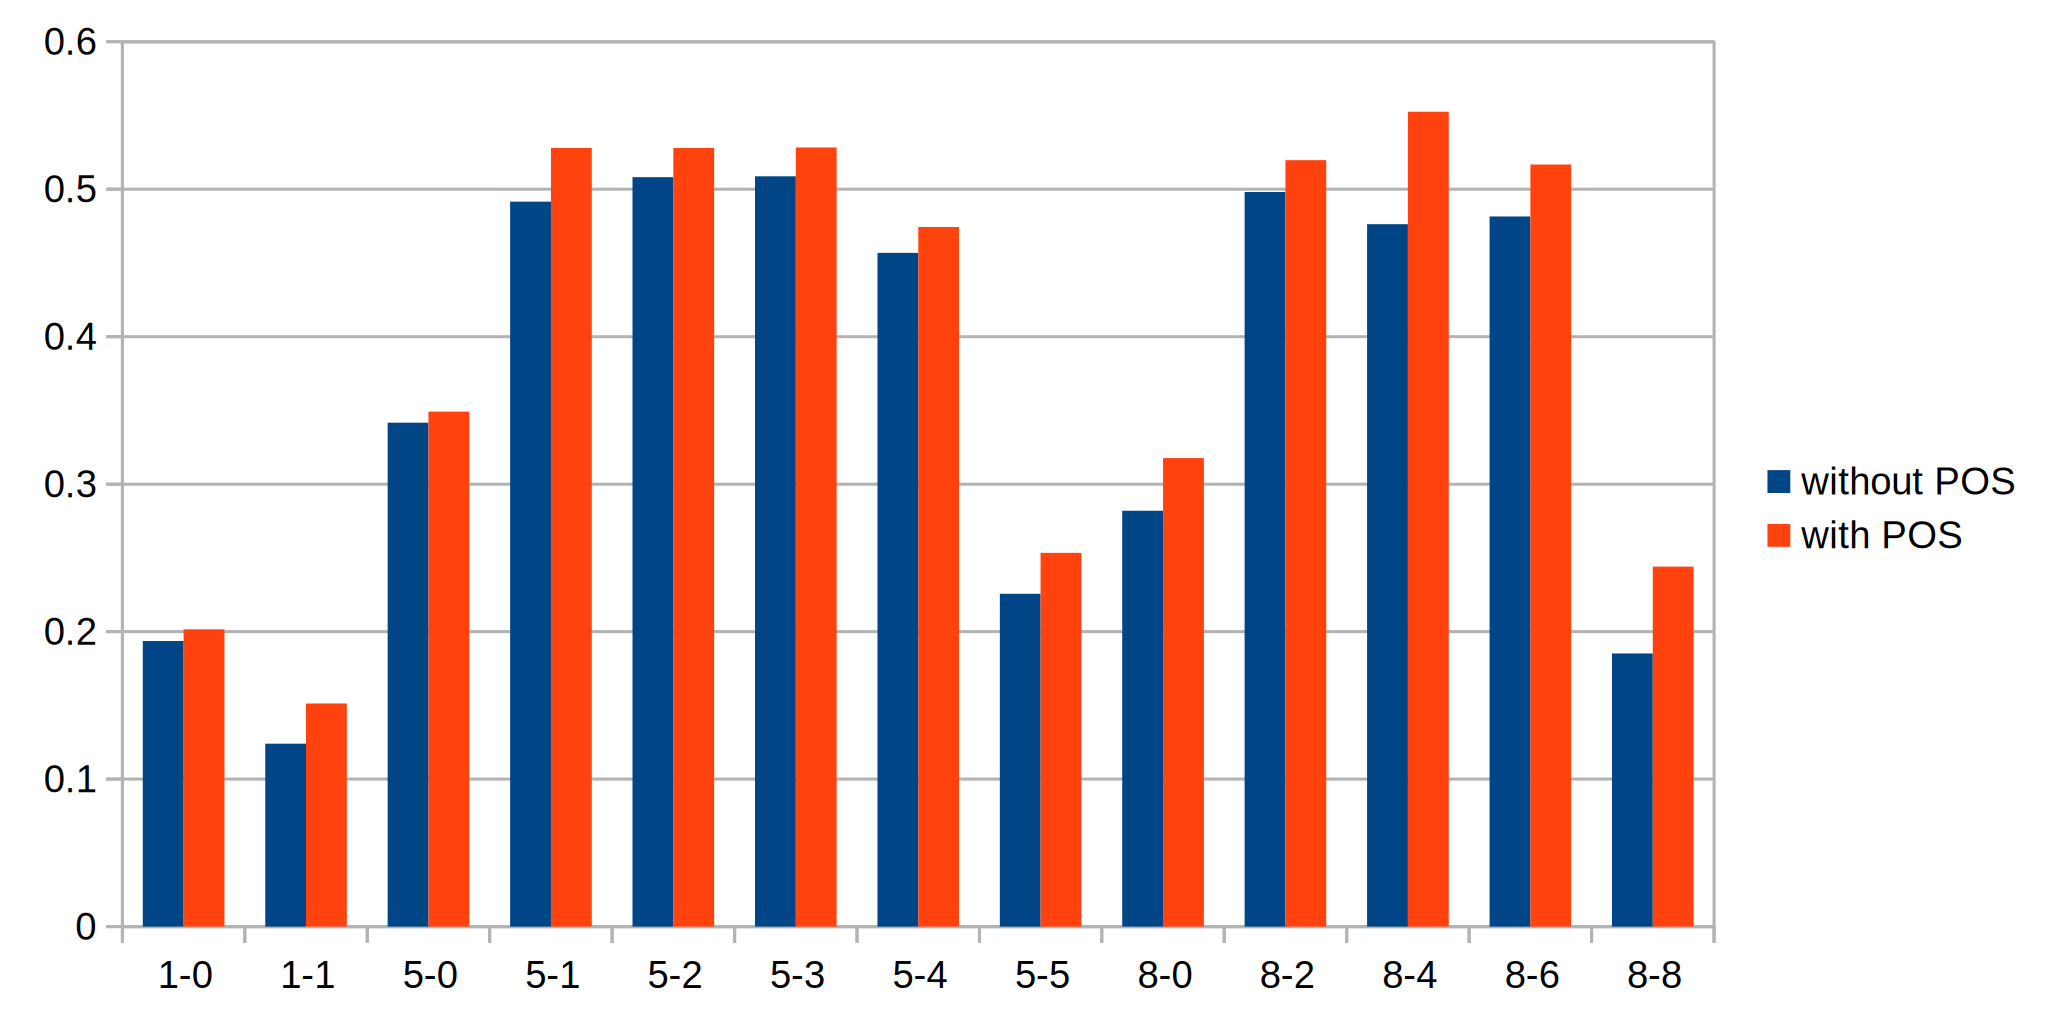
\includegraphics[width=0.7\textwidth]{img/window_pos_eval.png}
    \caption{Results for using POS tags as features (red bars) or not (blue bars). The F-score is plotted against different window sizes and punctuation positions. It is shown, that POS tags consistently improve the F-score.}
    \label{fig:window_pos_eval}
\end{figure}
The red bars show the results of using POS features and the blue bars show the result without POS tags as features.
Again, we see a consistent behavior: POS tags always help to increase the performance.

In Figure~\ref{fig:window_eval} you can see the combined results of the two experiments above.
\begin{figure}[ht]
    \centering
    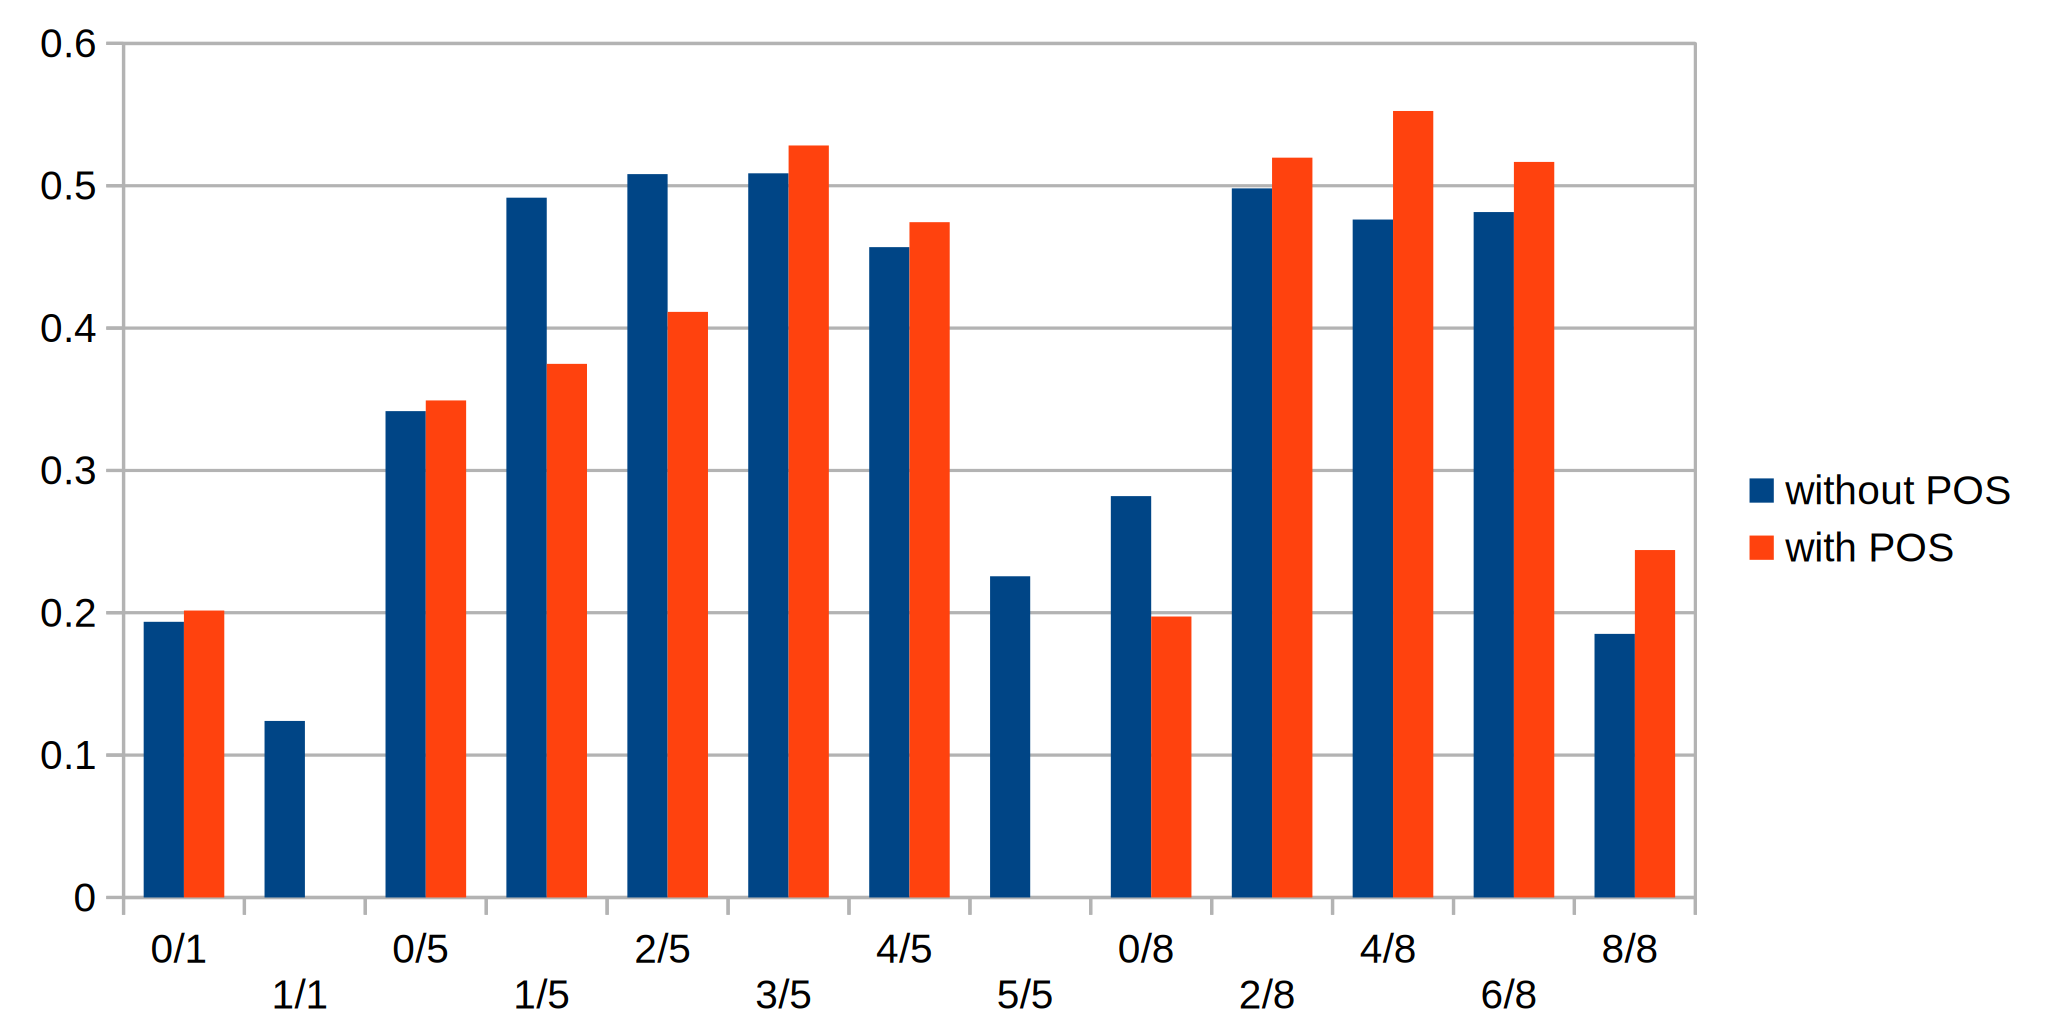
\includegraphics[width=0.9\textwidth]{img/window_eval.png}
    \caption{Results for using POS tags as features (red bars) or not (blue bars). The F-score is plotted against different window sizes and punctuation positions. Additionally, the \texttt{w} on the x-axis denotes whether Wikipedia is used in the training data set. The results show, that the best overall result can be achieved by using a window size of eight, a punctuation position of four, adding POS tags to the feature set, and not using Wikipedia in the training data set.}
    \label{fig:window_eval}
\end{figure}
Having a \texttt{w} behind the window size and punctuation position tuple means, that Wikipedia data was used in the training data set.
The different colors of the bars indicate again, if POS tag features were used.
The results show, that the best position for the punctuation is in the middle of the window.
We received the best overall result with a window size of eight and a punctuation position of four.
Also, Wikipedia data should not be used in the training data set and POS tags should be used as features.
Having this configuration, we obtain an F-score of 55.25\% for the lexical model.

In a last experiment we tried to reduce the dataset to a set, where all three classes are balanced, since the punctuation types in the data sets are not equally distributed.
Our experiments showed, that training on a balanced data set performs worse.
The main reason is probably, that the data set size is much smaller.